
\hypertarget{menu_edit}{}
\section{Edit}
\index{edit menu}

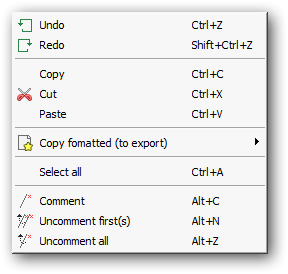
\includegraphics[scale=0.50]{./res/menu_edit.png}\\

\begin{scriptsize}\begin{tabularx}{\textwidth}{>{\hsize=0.4\hsize}X>{\hsize=0.7\hsize}X}\\
    \hline
    \textbf{Option} & \textbf{Description} \\
    \hline
    Undo & Undoes the last action \\
    Redo & Re-applies any actions undone using the Undo option \\
    Copy & Copies the selected text and places it in the Windows clipboard \\
    Cut & Cuts the selected text and places it in the Windows clipboard \\
    Paste & Places any text in the Windows clipboard at position indicated by the cursor within the file \\
    Copy formatted (to export) & \textit{\htmladdnormallink{See options ...}{\#menu\_edit\_copyformatted}} \\
    Select all & Selects the whole text contained in the file \\
    Comment & Adds comments to selected line(s) \\
    Uncomment firsts occurrence & Removes the first occurrence from a comment in the selected line(s) \\
    Uncomment all occurrence & Removes all occurrences from a comment in the selected line(s) \\
    \hline
  \end{tabularx}\end{scriptsize}


\hypertarget{menu_edit_copyformatted}{}
\subsection{Copy formatted (to export)}
\index{edit menu!copy formatted}

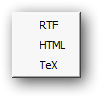
\includegraphics[scale=0.50]{./res/menu_edit_copyformated.png}\\

\begin{scriptsize}\begin{tabularx}{\textwidth}{>{\hsize=0.1\hsize}X>{\hsize=0.7\hsize}X}\\
    \hline
    \textbf{Option} & \textbf{Description} \\
    \hline
    RTF & Copies the selected text and places it in the Windows clipboard in Rtf format \\
    HTML & Copies the selected text and places it in the Windows clipboard in Html format \\
    TeX & Copies the selected text and places it in the Windows clipboard in TeX format \\
    \hline
  \end{tabularx}\end{scriptsize}
